In this section we aim to find out the effect of the lens height $h'$ on the coupling, where the lensed interface is made from the same material of the substrate. Here the guide end face is kept at the distance of $4\mu$m from the TLF and lens radius as a constant. Meanwhile the lens height $h'$ is varying from $0.4\mu$m to $3\mu$m. \\

Tab. \ref{tab:coupling_lensed_waveguide_height} shows 3 group of simulation results for lens radius of $R=2\mu$m, $2.5\mu$m and $3\mu$m and Fig. \ref{fig:coupling_lenses_curve_hxx} presents these results as curves. It can be seen that coupling efficiencies of each group are rising with the lens height increasing.  The coupling efficiency for the lens radius of $R=2.0\mu$m rises from $54\%$ at $h'=0.4\mu$m to $69\%$ at $h'=2.0\mu$m; the coupling efficiency for the lens radius of $R=2.5\mu$m rises from $53.4\%$ at $h'=0.4\mu$m to $68.8\%$ at $h'=2.4\mu$m; the coupling efficiency for the lens radius of $R=3.0\mu$m rises from $52.9\%$ at $h'=0.4\mu$m to $68.9\%$ at $h'=3.0\mu$m. Therefore, the most efficient lens configuration exists at the highest lens height when the radius of the lens is a constant. In another word a hemisphere lens is the best coupling configuration. \\

\begin{table}[!ht]
\caption{Coupling efficiency between TLF and lensed waveguide due to changing the lens height.}
\centering
\begin{tabular}{|c|c|c|c|}
\hline
\multirow{2}{*}{Height($\mu$m)}&\multicolumn{3}{c|}{Radius($\mu$m)}\\
\cline{2-4}
 			&	2&	2.5&	3\\
\hline
$0.4$&$54\%$&$53.4\%$&$52.9\%$\\
$0.6$&$58.35\%$&$57.4\%$&$56.9\%$\\
$0.8$&$57.3\%$&$56.7\%$&$56.3\%$\\
$1.0$&$60\%$&$58.8\%$&$57.8\%$\\
$1.2$&$60.7\%$&$59.1\%$&$57.9\%$\\
$1.4$&$61.7\%$&$59.9\%$&$58.8\%$\\
$1.6$&$65.1\%$&$62.7\%$&$60.7\%$\\
$1.8$&$62.9\%$&$60.9\%$&$59.9\%$\\
$2.0$&$69\%$  &  $66\%$&$63\%$\\
$2.2$&--------&$62.5\%$&$61.6\%$\\
$2.4$&--------&$68.8\%$&$64.4\%$\\
$2.6$&--------&--------&$66.7\%$\\
$2.8$&--------&--------&$64.8\%$\\
$3.0$&--------&--------&$68.9\%$\\
\hline
\end{tabular}
\label{tab:coupling_lensed_waveguide_height}
\end{table}
\begin{figure}[!ht]
\centering
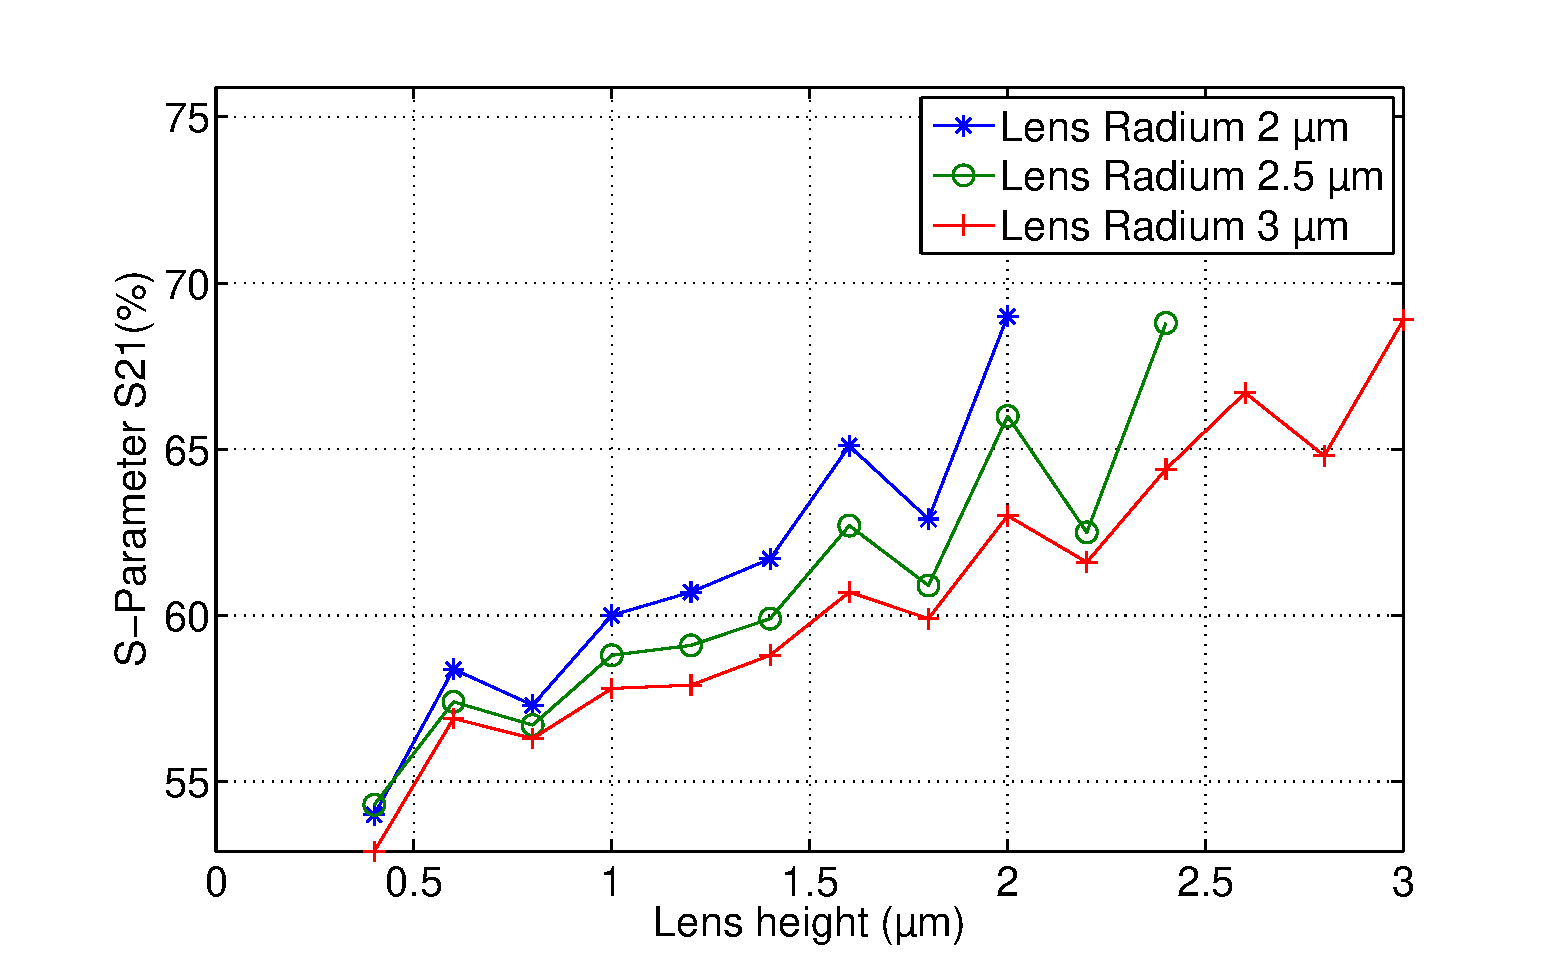
\includegraphics[width=0.7\textwidth]{bilder/s21_fix_lens_radium_hxx}
\caption{Coupling efficiency due to the variation of the lens height.}
\label{fig:coupling_lenses_curve_hxx}
\end{figure}
From simulation results it can be seen that the highest coupling efficiency in this case has significantly be improved in compare with the coupling efficiency of $51.3\%$ for regular buried waveguide in section \ref{sect:optim_lensed_regular}.\\

\begin{figure}[!ht]
\centering
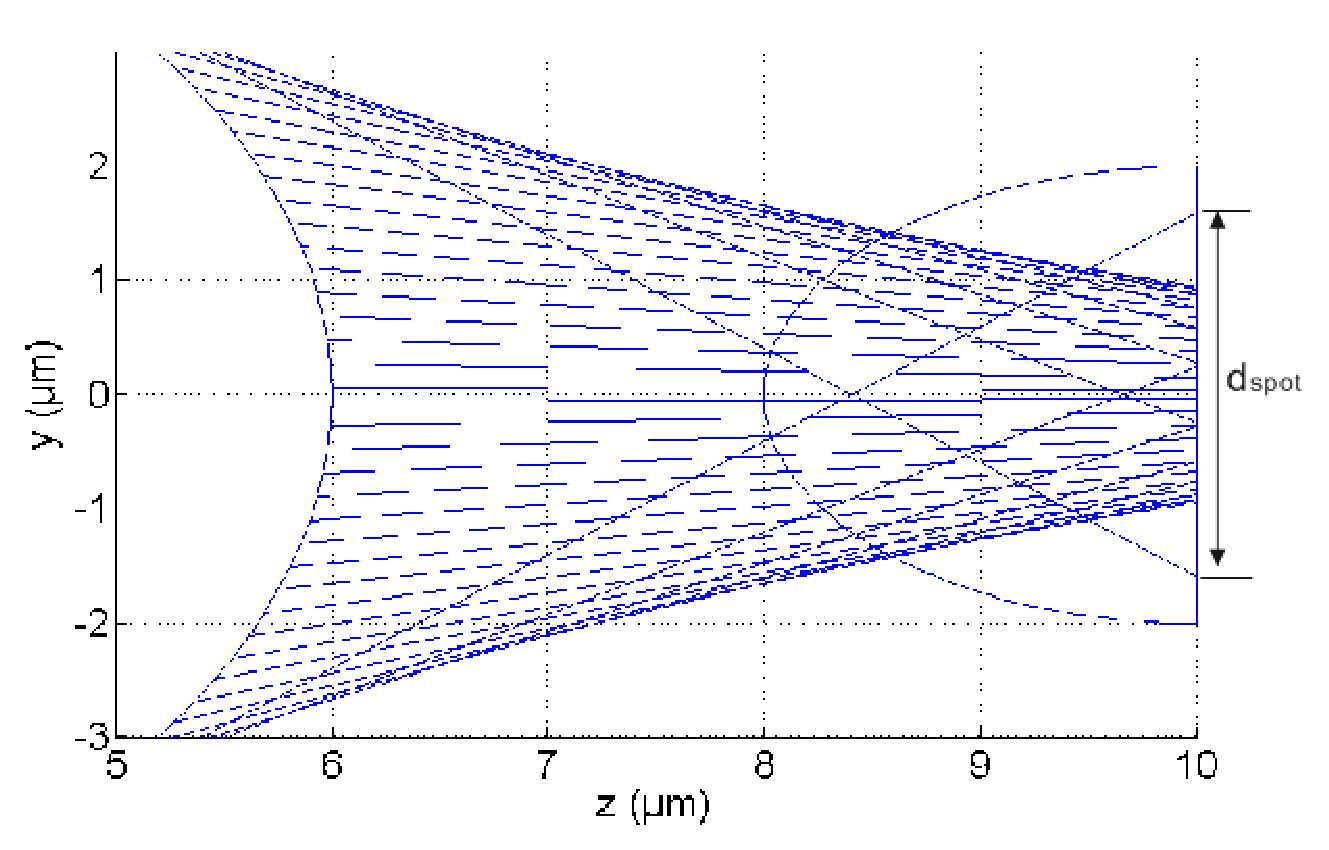
\includegraphics[width=0.7\textwidth]{bilder/beam_ray_without_refract}
\caption{Light propagates from TLF to waveguides without refraction in lens structure.}
\label{fig:matlab_coupling_lenses_rxx}
\end{figure}
\begin{figure}[!ht]
\centering
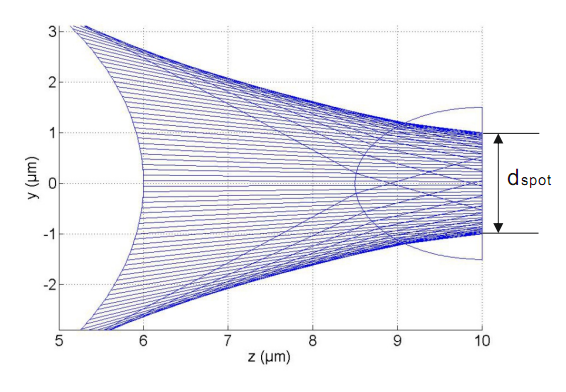
\includegraphics[width=0.7\textwidth]{bilder/beam_ray_refract}
\caption{ Light propagates from TLF to waveguides with refraction in lens structure.}
\label{fig:matlab_coupling_lenses_rxx2}
\end{figure} 
The reason of the efficiency change can be explained by lens theory with Fig. \ref{fig:matlab_coupling_lenses_rxx}-\ref{fig:matlab_coupling_lenses_rxx2}, which exhibits light propagating from TLF to the lens structure of the lensed waveguide. The left-hand arc presents the end of TLF and the right-hand half circle presents the lens structure of the lensed waveguide. $d_{spot}$ is the spot diameter at the waveguide end face. In Fig. \ref{fig:matlab_coupling_lenses_rxx} rays are not refracted by right-hand lens structure and $d_{spot}$ is about $2.4\mu$m. Fig. \ref{fig:matlab_coupling_lenses_rxx2} demonstrate that rays are refracted by right-hand lens, which has refractive index of $n=2.516$. In this case $d_{spot}$ is decreased less than $2.0\mu$m . That means, light power is confined in a smaller area and the coupling become more efficient. To verify this derivation we can check the spot size at the waveguide end face from CST MWS.\\

\begin{figure}[!ht]
\centering
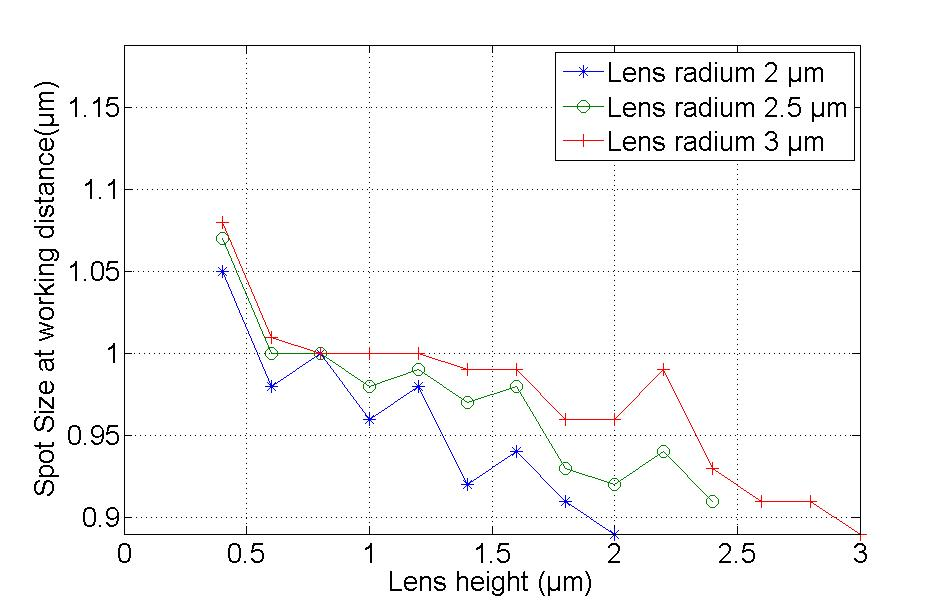
\includegraphics[width=0.7\textwidth]{bilder/spot_fix_lens_radium_hxx}
\caption{The spot size curve at lensed waveguide interface due to changing lens height, working frequency $f=282$THz.}
\label{fig:lensed_guide_spot_size_curve}
\end{figure}  
Fig. \ref{fig:lensed_guide_spot_size_curve} demonstrates spot size curves of 3 lens radii due to lens height at the end face of lensed waveguides. At the smallest lens height $h'=0.4\mu$m the spot size has highest values, about $1.05\mu$m for $R=2\mu$m, $1.07\mu$m for $R=2.5\mu$m and $1.08\mu$m for $R=3\mu$m. At the maximal lens height the spot size has minimum values, about $0.89\mu$m for $h'=2\mu$m and $R=2\mu$m, $0.91\mu$m for $h'=2.4\mu$m and $R=2.5\mu$m, $0.89\mu$m for $h'=3\mu$m and $R=3\mu$m. Curves in Fig. \ref{fig:lensed_guide_spot_size_curve} reveal that spot sizes changing agree well with the corresponding coupling efficiency inversely.\\
